% Search for all the places that say "PUT SOMETHING HERE".

\documentclass[11pt]{article}
\usepackage{amsmath,textcomp,amssymb,graphicx,enumerate,hyperref,enumitem,mathtools,tikz-qtree,listings,chemformula,bm,graphicx,grffile,gensymb,physics,amssymb,datetime,siunitx}
\graphicspath{{/Users/jonathansun5/Documents/Fall 2017/MCB 166/Homeworks/HW 3/Screen Shot 2017-10-14 at 6.38.44 PM.png} {/Users/jonathansun5/Documents/Fall 2017/MCB 166/Homeworks/HW 3/Screen Shot 2017-10-14 at 6.40.12 PM.png} {/Users/jonathansun5/Documents/Fall 2017/MCB 166/Homeworks/HW 3/Screen Shot 2017-10-14 at 7.07.44 PM.png} {/Users/jonathansun5/Documents/Fall 2017/MCB 166/Homeworks/HW 3/Screen Shot 2017-10-14 at 7.10.16 PM.png} {/Users/jonathansun5/Documents/Fall 2017/MCB 166/Homeworks/HW 3/Screen Shot 2017-10-16 at 6.22.55 PM.png}}

\makeatletter
\newcommand{\leqnos}{\tagsleft@true\let\veqno\@@leqno}
\newcommand{\reqnos}{\tagsleft@false\let\veqno\@@eqno}
\reqnos
\makeatother

\def\Name{Jonathan Sun}  % Your name
\def\SID{25020651}  % Your student ID number
\def\Homework{3} % Number of Homework
\def\Session{Fall 2017}


\title{MCB166 --- \Session --- Problem Set \Homework}
\author{\Name, SID \SID}
\markboth{MCB166 --- \Session --- Problem Set \Homework --- \Name}{MCB166 --- \Session --- Problem Set \Homework --- \Name}
\pagestyle{myheadings}
\newdate{date}{17}{10}{2017}
\date{\displaydate{date}}

\def\endproofmark{$\Box$}
\newenvironment{proof}{\par{\bf Proof:}}{\endproofmark\smallskip}

\usepackage[margin=1in]{geometry}



\begin{document}
\maketitle

\newpage
\begin{enumerate}[label=\arabic*.]
\item
The unicellular organism \textit{Paramecium caudatum} shows a resting potential (RP) and an action potential (AP) that are similar in many respects to corresponding neural potentials. With the cell in ``typical pond water,'' the following measurements were made with an intracellular electrode:
\begin{center}
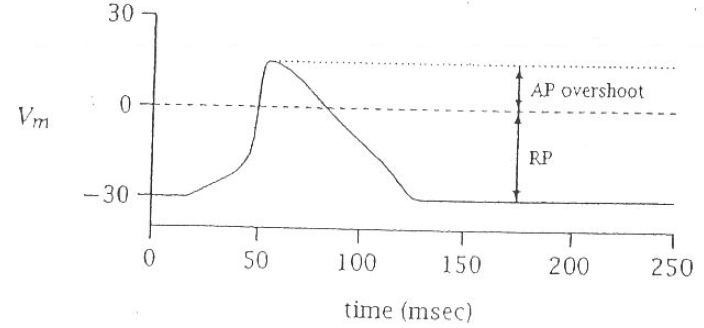
\includegraphics[width=0.75\textwidth]{/Users/jonathansun5/Documents/Fall 2017/MCB 166/Homeworks/HW 3/Screen Shot 2017-10-14 at 6.38.44 PM.png}
\end{center}
If one varies $[\ch{K+}]_{\text{out}}$ only, or $[\ch{Ca^{2+}}]_{\text{out}}$ only, one observes the following:
\begin{center}
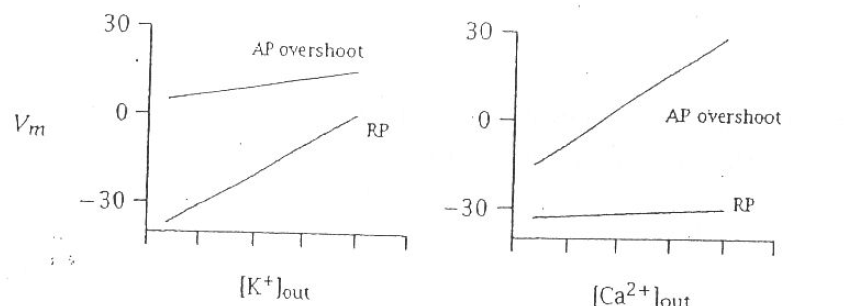
\includegraphics[width=0.75\textwidth]{/Users/jonathansun5/Documents/Fall 2017/MCB 166/Homeworks/HW 3/Screen Shot 2017-10-14 at 6.40.12 PM.png}
\end{center}
In the following questions, assume that the membrane of \textit{P. caudatum} is normally permeable only to \ch{K+}, \ch{Ca^{2+}}, and water.
\begin{enumerate}[label=(\alph*)]
\item
In the resting state, which of these is true? Explain concisely.
\begin{enumerate}[label=\roman*.]
\item
$P_{\ch{K}} > P_{\ch{Ca}}$
\item
$P_{\ch{K}} = P_{\ch{Ca}}$
\item
$P_{\ch{K}} < P_{\ch{Ca}}$
\end{enumerate}
\vspace*{1\baselineskip}
The correct answer is \textbf{i. $P_{\ch{K}} > P_{\ch{Ca}}$}. This is because the slope for the resting potential in the $V_m$ vs. $[\ch{K+}]_{\text{out}}$ graph is much greater than the slope for the resting potential in the $V_m$ vs. $[\ch{Ca^{2+}}]_{\text{out}}$ graph even though they both started at around $V_m = -30 \text{mV}$. Therefore, the $V_m$ of the resting potential as $[\ch{K+}]_{\text{out}}$ increses is much higher than the $V_m$ of the resting potentil as $[\ch{Ca^{2+}}]_{\text{out}}$. This means that the resting membrane potential depends more on $[\ch{K+}]_{\text{out}}$ than $[\ch{Ca^{2+}}]_{\text{out}}$.
\\



\item
Which is true during the peak of the AP? Explain concisely.
\vspace*{1\baselineskip}
\\
During the peak of the action potential, $P_{\ch{K}} < P_{\ch{Ca}}$ because the $V_m$ for $[\ch{Ca^{2+}}]_{\text{out}}$ increases a lot more than the $V_m$ for $[\ch{K+}]_{\text{out}}$, which means that $P_{\ch{Ca}}$ is influenced a lot more than $P_{\ch{K}}$. This means that the action potential depends more on $[\ch{Ca^{2+}}]_{\text{out}}$ than $[\ch{K+}]_{\text{out}}$.
\\



\item
Compared to the ionic concentrations of ``typical pond water,'' is $[\ch{K+}]_{\text{in}}$ greater than, equal to, or less that $[\ch{K+}]_{\text{out}}$? Explain.
\vspace*{1\baselineskip}
\\
Compared to the ionic concentrations of ``typical pond water,'' $[\ch{K+}]_{\text{in}} > [\ch{K+}]_{\text{out}}$. This is because in part (a) we have determined that at the resting potential, $P_{\ch{K}} > P_{\ch{Ca}}$, which means that the resting potential depends more on $[\ch{K+}]_{\text{out}}$ than $[\ch{Ca^{2+}}]_{\text{out}}$. Therefore, we will disregard $[\ch{Ca^{2+}}]_{\text{out}}$ from our calculations. Since $V_{\text{rest}} \approx -30 \text{mV}$ and this is close to $E_{\ch{K}}$, I know that I should get a negative number for $E_{\ch{K}}$. Calculating for $E_{\ch{K}}$ we get:
\begin{align*}
V_{\text{rest}} \approx E_{\ch{K}} = \frac{RT} {zF} \ln{\frac{P_{\ch{K}}[\ch{K+}]_{\text{out}}} {P_{\ch{K}}[\ch{K+}]_{\text{in}}}} \approx -30 \text{mV}
\end{align*}
Since the only way for $\frac{RT} {zF} \ln{\frac{P_{\ch{K}}[\ch{K+}]_{\text{out}}} {P_{\ch{K}}[\ch{K+}]_{\text{in}}}}$ to be negative is for the numerator of the natural log to be smaller than the denominator of the natural log, this means that $[\ch{K+}]_{\text{in}} > [\ch{K+}]_{\text{out}}$.
\\



\item
Compare also $[\ch{Ca^{2+}}]_{\text{in}}$ with $[\ch{Ca^{2+}}]_{\text{out}}$.
\vspace*{1\baselineskip}
\\
Compared to the ionic concentrations of ``typical pond water,'' $[\ch{Ca^{2+}}]_{\text{in}} < [\ch{Ca^{2+}}]_{\text{out}}$. This is because in part (b) we have determined that at the action potential, $P_{\ch{K}} < P_{\ch{Ca}}$, which means that the action potential depends more on $[\ch{Ca^{2+}}]_{\text{out}}$ than $[\ch{K+}]_{\text{out}}$. Therefore, we will disregard $[\ch{K+}]_{\text{out}}$ from our calculations. Since $V_{\text{AP}} \approx +15 \text{mV}$ and this is close to $E_{\ch{K}}$, I know that I should get a negative number for $E_{\ch{K}}$. Calculating for $E_{\ch{Ca}}$ we get:
\begin{align*}
V_{\text{AP}} \approx E_{\ch{Ca}} = \frac{RT} {zF} \ln{\frac{P_{\ch{Ca}}[\ch{Ca^{2+}}]_{\text{out}}} {P_{\ch{Ca}}[\ch{Ca^{2+}}]_{\text{in}}}} \approx +15 \text{mV}
\end{align*}
Since the only way for $\frac{RT} {zF} \ln{\frac{P_{\ch{Ca}}[\ch{Ca^{2+}}]_{\text{out}}} {P_{\ch{Ca}}[\ch{Ca^{2+}}]_{\text{in}}}}$ to be positive is for the numerator of the natural log to be greater than the denominator of the natural log, this means that $[\ch{Ca^{2+}}]_{\text{in}} < [\ch{Ca^{2+}}]_{\text{out}}$.
\\



\item
When the posterior end of the organism is mechanically tapped, the membrane transiently hyperpolarizes. What permeability change(s) might be responsible? Explain.
\vspace*{1\baselineskip}
\\
When the membrane transiently hyperpolarizes, this may be caused by the increase in $P_{\ch{K}}$. This is because at resting potential, we found that $P_{\ch{K}} > P_{\ch{Ca}}$ and so the increase in $P_{\ch{K}}$ would have more effect than the decrease in $P_{\ch{Ca}}$ for hyperpolarization.
\end{enumerate}



\newpage
\item
\begin{enumerate}[label=(\alph*)]
\item
Briefly state the assumptions for the constant field model.
\vspace*{1\baselineskip}
\\
The constant field model assumes that ion movement within the membrane obeys the Nernst-Planck equation, ions move across the membrane independently without interacting with each other, and the electric field in the membrane is constant (the electric potential drops linearly across the membrane).
\\



\item
Sketch approximately the \textit{I-V} relations predicted by the constant field model for various ratios of intracellular and extracellular ion concentrations, i.e., when $\frac{[\ch{C}]_{\text{in}}} {[\ch{C}]_{\text{out}}} = 0\text{, } 0.1\text{, } 1\text{, } 30\text{, or } \infty$.
\begin{center}
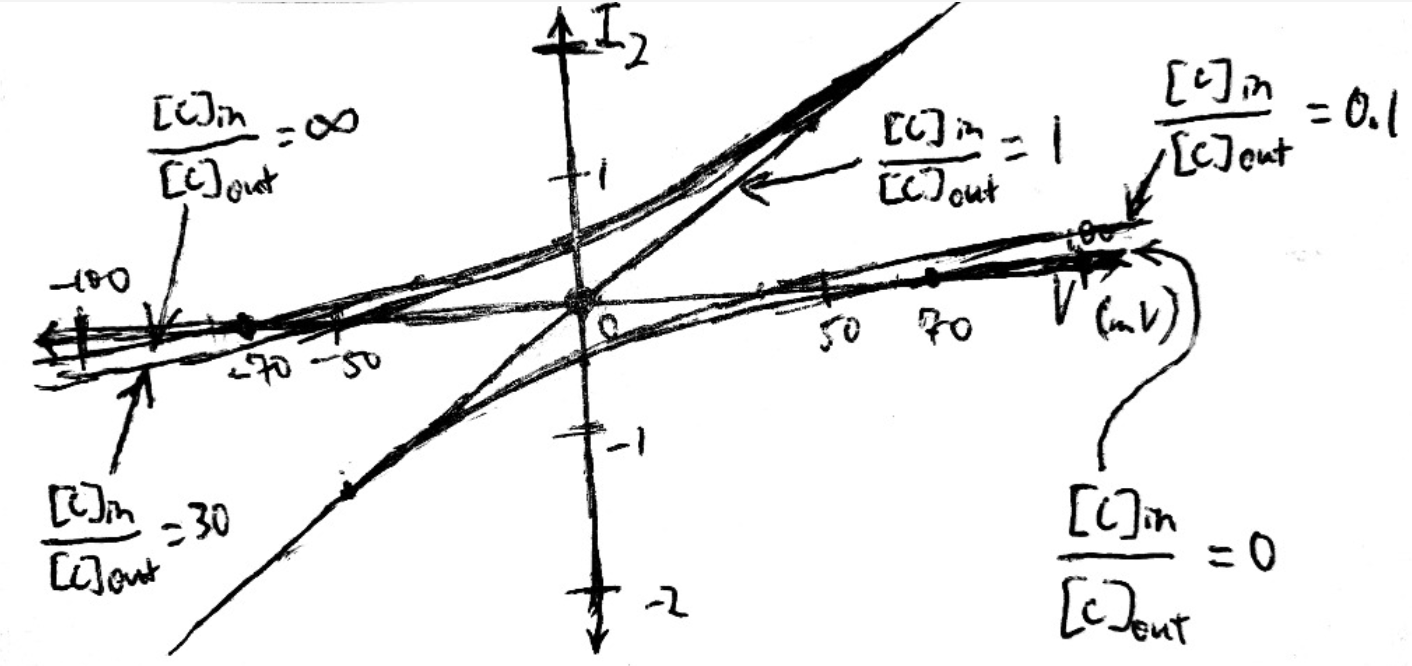
\includegraphics[width=0.75\textwidth]{/Users/jonathansun5/Documents/Fall 2017/MCB 166/Homeworks/HW 3/Screen Shot 2017-10-16 at 6.22.55 PM.png}
\end{center}



\item
Using the data provided in the figure below, calculate the ratio of $P_{\ch{Na}} / P_{\ch{K}}$ that predicts the resting potential as a function of $[\ch{K}]_{\text{out}}$ for the \textit{Myxicola} neuron. Note: $[\ch{Na+}]_{\text{out}} = 430 \text{mM}$, $[\ch{Na+}]_{\text{in}} = 12 \text{mM}$, $[\ch{K+}]_{\text{in}} = 270 \text{mM}$, and $P_{\ch{Cl}} = 0$.
\begin{center}
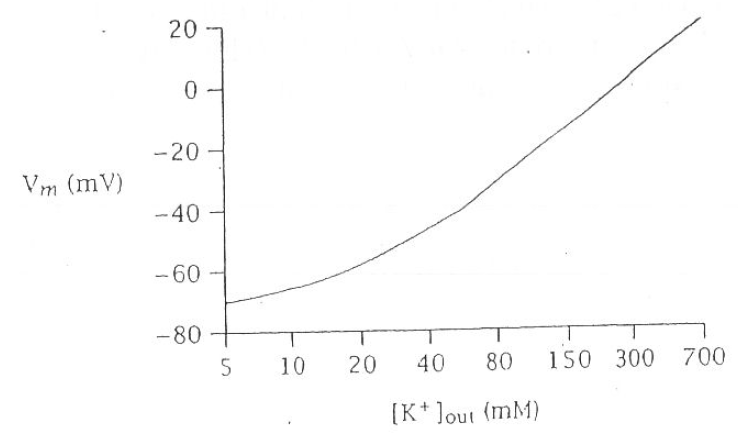
\includegraphics[width=0.75\textwidth]{/Users/jonathansun5/Documents/Fall 2017/MCB 166/Homeworks/HW 3/Screen Shot 2017-10-14 at 7.07.44 PM.png}
\end{center}



\end{enumerate}













\newpage
\item
The instantaneous and steady-state $I-V$ relations of a neuron obtained from voltage-clamp experiments are shown below:
\begin{center}
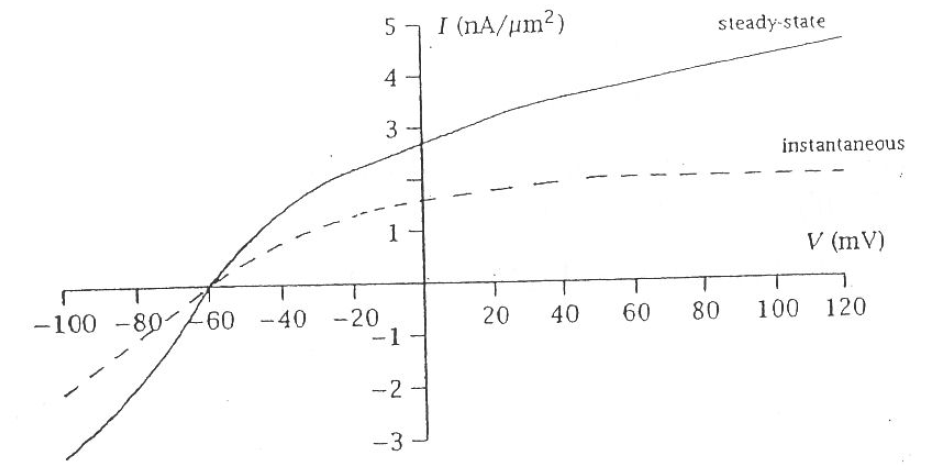
\includegraphics[width=0.75\textwidth]{/Users/jonathansun5/Documents/Fall 2017/MCB 166/Homeworks/HW 3/Screen Shot 2017-10-14 at 7.10.16 PM.png}
\end{center}
The time-dependent current follows first-order kinetics with the time constant $\tau = 0.1$ sec.
\begin{enumerate}[label=(\alph*)]
\item
Draw the membrane current with respect to time after the membrane voltage is stepped from $V_H = -60 \text{mV}$ to $V_c = 0 \text{mV}$ and to $V_c = -80 \text{mV}$. Label the current and time axes with the appropriate units.






\item
Repeat (a) after the membrane voltage is stepped from $V_H = +50 \text{mV}$ to $V_c = +100 \text{mV}$.












\end{enumerate}




\end{enumerate}
\end{document}
